\chapter{Parallélisations et optimisations}
\label{chap:parallelisations_et_optimisations}


Dans ce chapitre, nous décrivons l’implémentation sur un ou plusieurs
accélérateurs de la méthode Galerkin Discontinue (GD) décrite au chapitre \ref{chap:implementation}.
Pour cela, nous utilisons la bibliothèque OpenCL
(pour « \textit{Open Computing Language} ») \cite{opencl} qui permet d’exploiter la puissance
de calcul des accélérateurs (cartes graphiques, processeurs multi-cœurs, coprocesseurs, \textit{etc}.) produits par divers constructeurs
(NVidia, AMD, Intel) et compatibles avec différents systèmes d’exploitation (Linux, Windows, Mac OS).

La puissance des cartes graphiques récentes permet de réaliser des calculs
de façon massivement parallèle. Ces GPGPU (pour « \textit{General Purpose Graphic Processing Unit} »), ou plus simplement GPU, possèdent une puissance crête élevée, de l’ordre
de plusieurs téraflops. Ce type de matériel est très utilisé dans la simulation numérique.
Nous les retrouvons par exemple dans la résolution des équations de Maxwell
\cite{cabel:inria-00583617, Klockner:2009:NDG:1613335.1613429},
de Vlasov-Maxwell \cite{crestetto:hal-00731021}, dans la simulation
de gaz et fluides \cite{devuyst:hal-00687566, helluy:hal-00957020},
et bien d'autres domaines.
L'implémentation GPU a initialement été réalisée en C++ en utilisant la bibliothèque
OpenCL au cours de la thèse de Strub \cite{strub:tel-01651258}, à partir du code non parallèle
FemGD développé à l'ONERA de Toulouse \cite{Coh-Fer-Per-2006-1}.

Afin de pouvoir traiter des volumes de données importants, la méthode GD est
également parallélisée sur plusieurs accélérateurs à l'aide d'une implémentation du standard
MPI (« \textit{Message Passing Interface} ») \cite{10.1007/978-3-0348-8534-8_21}. MPI offre la possibilité de lancer plusieurs
processus qui effectuent les calculs sur différentes parties du maillage
et communiquent par un système de messages.

Cette implémentation GPU est aussi exploitable sur un processeur multi-cœurs
(CPU) plus classique. Ces derniers ont beaucoup évolué au cours des années passées
pour être aujourd'hui composés de plusieurs dizaines de cœurs logiques cadencés
à des fréquences supérieures à celles des GPU. Cependant, de par leur architecture
distincte de celle des GPU, une implémentation spécifique aux CPU doit être
développée afin de les exploiter au mieux.

Dans un premier temps, nous présenterons la parallélisation OpenCL des calculs
sur GPU ainsi que la stratégie asynchrone
de parallélisation MPI.
Ensuite nous décrirons les adaptations effectuées afin d'en améliorer
les performances sur CPU.
Enfin, nous présenterons une méthode d'adaptation de l'ordre d'interpolation
spatiale appliquée aux mailles du maillage dans le but de réduire le temps
de simulation en optimisant l'échantillonnage du domaine de calcul.
\\


\section{La bibliothèque OpenCL}
\label{sect:librairie_opencl}

OpenCL est une interface de programmation
(ou API pour « \textit{Application Programming Interface} ») maintenue par le Khronos Group
\cite{opencl}, qui gère aussi le standard graphique OpenGL.
Cette API a initialement été créée par Apple, puis confiée à Khronos en 2008,
dans l’espoir qu’elle devienne un standard. Les différents constructeurs
d'accélérateurs (NVidia, AMD, Intel) ont développé et maintiennent
des pilotes permettant d’utiliser OpenCL pour paralléliser des calculs sur
leurs matériels.

Dans l’abstraction OpenCL, le processeur appelé hôte (ou « \textit{host} ») exécute les
instructions du programme principal et assure la soumission des calculs sur les
périphériques de calculs ainsi que les tâches annexes (pré- et post-traitement
des données, \textit{etc}.).
\\

\subsection{Les périphériques OpenCL}
\label{ssect:peripheriques_opencl}

Les périphériques de calculs (ou accélérateurs, ou « \textit{devices} ») exécutent les calculs
parallèles programmés sous forme de fonctions à l'aide d'un langage dérivé du C.
Une telle fonction est appelée noyau (ou « \textit{kernel} »). L'exécution d'un kernel
par un périphérique ou le transfert de données entre le périphérique et l'hôte
sont appelés des tâches. La soumission d'une tâche est effectuée via une file
d’attente.

Du point de vue de l’exécution d’un kernel, le périphérique est vu sous
la forme d’un ensemble d’unités de travail appelées « \textit{work-items} », rassemblés
en groupes de travail appelés « \textit{work-groups} ». Un kernel a aussi accès à plusieurs
espaces mémoire (figure \ref{img:opencl_device}). En particulier, tous les
work-items d'un même work-group ont accès à un espace mémoire partagé réservé.
\\


L’exécution des tâches peut être gérée de plusieurs manières :
elles peuvent être soumises de manière synchrone ou asynchrone.
Dans le cas synchrone, les tâches sont exécutées dans l’ordre de soumission et
le programme hôte est stoppé durant l’exécution d'une tâche.
Ce mode de soumission est généralement utilisé en phase de développement
pour se soustraire des éventuelles erreurs de synchronisation.

Dans le cas asynchrone, chaque tâche est associée à un évènement qui permet
de consulter son statut d’exécution : en attente, soumise, en cours d’exécution
ou terminée. Contrairement au mode synchrone, le programme hôte continue son
exécution sans interruption jusqu'à rencontrer un point de synchronisation demandé
par l'utilisateur. Afin de garantir le bon enchaînement des calculs,
l’exécution d’une tâche peut être conditionnée par la terminaison d’un ensemble
de tâches à l’aide des évènements qui leur sont associés. Ces dépendances entre
les évènements sont représentées au moyen d’un graphe acyclique direct appelé
graphe de tâches.
\\

\begin{figure}[h]
	\begin{center}
		\caption{
			\label{img:opencl_device}
			Schéma d'un périphérique OpenCL présentant des work-items
			regroupés en work-groups.
		}
		
		\pgfdeclarelayer{wilayer}
		\pgfdeclarelayer{wglayer}
		\pgfsetlayers{main,wglayer,wilayer}
		
		\tikzstyle{wd}=[
			minimum height = 1em, minimum width = 1em, outer sep = 0.1em
		]
		\tikzstyle{wi}=[wd,
			draw = blue, fill = blue!20,
		]
		
		\tikzstyle{brace}=[
			decoration={brace, raise = 0.1em}, decorate
		]
		\tikzstyle{bracetxt}=[
			above = 0.3em, midway
		]

		\tikzstyle{wg}=[
			draw = yellow, fill = yellow!20, minimum width = 7em,
			inner sep = 0.5em, outer sep = -0.1em
		]
		\tikzstyle{wgh}=[wg,
			fill = yellow!40, inner sep = 0.3em
		]
		\tikzstyle{wgwrap}=[
			inner sep = 0.1em
		]
		
		\tikzstyle{gmem}=[
			draw = black, fill = gray!20, minimum width = 24em, minimum height = 2em
		]
		\tikzstyle{lmem}=[gmem,
			minimum width = 7em
		]
		
		\begin{tikzpicture}
			\begin{pgfonlayer}{wilayer}
				\node (wi11) [wi] {};
				\node (wi12) [wi, right = 0.1em of wi11] {};
				\node (wi1d) [wd, right = 0.1em of wi12] {\small $\dots$};
				\node (wi1k) [wi, right = 0.1em of wi1d] {};
				\draw[brace] (wi11.north west) -- (wi1k.north east)
					node[bracetxt, name = b1]{\tiny $k$ work-items};
				\node (wi21) [wi, right = 1.6em of wi1k] {};
				\node (wi22) [wi, right = 0.1em of wi21] {};
				\node (wi2d) [wd, right = 0.1em of wi22] {\small $\dots$};
				\node (wi2k) [wi, right = 0.1em of wi2d] {};
				\draw[brace] (wi21.north west) -- (wi2k.north east)
					node[bracetxt, name = b2]{\tiny $k$ work-items};
				\node (win1) [wi, right = 3.2em of wi2k] {};
				\node (win2) [wi, right = 0.1em of win1] {};
				\node (wind) [wd, right = 0.1em of win2] {\small $\dots$};
				\node (wink) [wi, right = 0.1em of wind] {};
				\draw[brace] (win1.north west) -- (wink.north east)
					node[bracetxt, name = bk]{\tiny $k$ work-items};
			\end{pgfonlayer}
			
			\begin{pgfonlayer}{wglayer}
				\node (wg1) [wg, fit = (wi11)(wi1k)(b1)] {};
				\node (wg1h) [wgh, above = 0em of wg1] {\small work-group $1$};
				\node (wg2) [wg, fit = (wi21)(wi2k)(b2)] {};
				\node (wg2h) [wgh, above = 0em of wg2] {\small work-group $2$};
				\node (wgd) [wd, right = 0.1em of wg2] {$\dots$};
				\node (wgn) [wg, fit = (win1)(wink)(bk)] {};
				\node (wgnh) [wgh, above = 0em of wgn] {\small work-group $n$};

				\node (wgw1) [wgwrap, fit = (wg1)(wg1h)] {};
				\node (wgw2) [wgwrap, fit = (wg2)(wg2h)] {};
				\node (wgwn) [wgwrap, fit = (wgn)(wgnh)] {};
				\node (wgc) [fit = (wgw1)(wgw2)(wgwn)] {};
				
				\node (lmem1) [lmem, above = 1em of wgw1] {\tiny Mémoire locale (ko)};
				\node (lmem2) [lmem, above = 1em of wgw2] {\tiny Mémoire locale (ko)};
				\node (lmemd) [right = 0.1em of lmem2] {$\dots$};
				\node (lmemn) [lmem, above = 1em of wgwn] {\tiny Mémoire locale (ko)};
	
				\node (gmem) [gmem, below = 1em of wgc] {\small Mémoire globale (Go)};
				\node (gmem1) [below = 1.4em of wgw1] {};
				\node (gmem2) [below = 1.4em of wgw2] {};
				\node (gmemn) [below = 1.4em of wgwn] {};
				
				\draw[arrows={-latex}] (wgw1.north) -- (lmem1.south);
				\draw[arrows={-latex}] (wgw2.north) -- (lmem2.south);
				\draw[arrows={-latex}] (wgwn.north) -- (lmemn.south);
				
				\draw[arrows={-latex}] (wgw1.south) -- (gmem1.north);
				\draw[arrows={-latex}] (wgw2.south) -- (gmem2.north);
				\draw[arrows={-latex}] (wgwn.south) -- (gmemn.north);
			\end{pgfonlayer}
		\end{tikzpicture}
	\end{center}
\end{figure}


\subsection{La mémoire OpenCL}
\label{ssect:memoire_opencl}


Dans l'API OpenCL, la mémoire d'un périphérique est constituée de différentes parties. Par défaut, une variable définie dans un kernel est allouée dans l'espace privé
du work-item (aussi identifiable par le préfixe facultatif
\verb|__private|).
Cette mémoire est allouée pour chaque work-item et demeure la plus rapide.

Nous disposons aussi d'une mémoire constante (identifiée par le préfixe
\verb|__constant|).
Cette mémoire est d’accès rapide et accessible par tous les work-items. Les données
de cet espace sont définies et allouées lors de la compilation des kernels
et en lecture seule : leurs valeurs ne peuvent pas être changées lors de l’exécution.

Ensuite, chaque work-group a accès une mémoire locale (identifiée par le préfixe \verb|__local|). Les accès à cette  mémoire cache sont très rapides, mais les
valeurs qui y sont stockées ne sont accessibles que par les work-items du
work-group et sont perdues à la fin de l’exécution du kernel. La taille
de cette mémoire est petite, de l’ordre de quelques dizaines de kilo-octets, et
a pour but d'y stocker les données temporaires partagées au sein du work-group.

Enfin, un périphérique contient une mémoire globale (identifiée par le préfixe \verb|__global|). Celle-ci est de l’ordre de quelques gigaoctets dans le cas
d’un GPU et correspond à la mémoire vive du nœud dans le cas d'un CPU.
Cette mémoire est accessible par tous les work-items exécutant un kernel.
Les lectures et écritures y sont relativement lentes. De plus, l’efficacité des
accès à cette mémoire est conditionnée par leur ordonnancement. La façon la plus
efficace de procéder est d’y accéder de manière « coalescente » : c'est à dire
lorsque les work-items dont les numéros se suivent accédent à des données rangées
de manière contiguë et dans le même ordre.
\\

\subsection{Les kernels OpenCL}
\label{ssect:kernels_opencl}

Les sources des kernels peuvent être dynamiquement construites par le programme hôte
et compilées au cours de l’exécution.
Ceci nous permet d’y inclure des constantes qui facilitent leur programmation.

Lors de l’exécution d’un kernel par le périphérique OpenCL, nous avons aussi
accès à des données contextuelles qui permettent de piloter la parallélisation.
Nous pouvons par exemple connaitre le numéro du work-group et le numéro du
work-item. Ces données permettent alors de paralléliser les calculs de la
manière souhaitée.

Le nombre de work-items et la taille des work-groups associés à l’exécution d’un
kernel sont spécifiés lors de la soumission de la tâche à la file d’attente.
Tous les work-items exécutent alors le même kernel en parallèle. Cependant,
dans le cas d'un GPU qui possède une architecture SIMD (pour
«~\textit{Simple Instruction, Multiple Data}~»), contrairement aux CPU
qui possèdent une architecture MIMD (pour «~\textit{Multiple Instructions, Multiple Data}~»),
les work-items d’un même work-group partagent la même unité d’instructions,
c'est-à-dire que les instructions conditionnelles conduisent
à l’exécution successive de toutes les branches et seules les écritures sont
désactivées dans les branches rejetées. Ainsi, nous devons limiter au maximum
le nombre de branches présentes dans les kernels.
\\



\section{Implémentation GPU}
\label{sect:implementation_gpu}

Initialement, l’implémentation de l’algorithme GD a plus spécifiquement été adaptée
aux GPU. Ce type de périphérique possède un volume de mémoire limité. Afin de
réduire le volume de données, certains paramètres constants sont donc calculés
lorsque requis. De plus, il est nécessaire d’utiliser les ressources
de mémoire locale pour y stocker les résultats intermédiaires, mais aussi
certaines données auxquelles l’accès est fréquent.

\begin{remark}
	Nous présentons dans cette section les kernels optimisés
	pour hexaèdres. Le solveur possède aussi les kernels
	génériques qui permettent d'effectuer des calculs
	sur tétraèdres. Ces kernels génériques sont semblables
	aux kernels optimisés, mais sans tenir compte des
	simplifications liées aux propriétés des fonctions
	de base.
	\\
\end{remark}


\subsection{Zones homogènes}
\label{ssect:zones_homogenes}

Un GPU est composé de plusieurs milliers de work-items travaillant
en parallèle. Afin que leur utilisation soit optimale, l'exécution d'un kernel
doit solliciter tous les work-items disponibles. Ce maximum ne peut pas être atteint
avec un kernel traitant une seule ou peu de mailles à la fois. Les mailles sont
donc réparties dans des zones homogènes. Chaque zone contient une unique géométrie
de maille ainsi qu’une même base d’approximation.

Cette répartition en zones homogènes nous permet de spécifier et simplifier les
kernels de calcul afin de limiter au maximum les branches conditionnelles
qui dégradent les performances.
Chaque zone de maillage est transformée en tableaux de données dans la phase de
pré-traitement et à destination des kernels OpenCL.
Ainsi, les données géométriques se résument en $3$ tableaux :
les coordonnées des nœuds (réels), la définition des mailles par les indices de leurs
sommets (entiers) et la connectivité entre les faces des mailles voisines (entiers).
La transformation géométrique associée à chaque maille, les coordonnées des points
d'interpolation et la valeur des fonctions de base sont recalculées dès que
nécessaires.


\subsubsection{Stockage coalescent}
\label{sssect:zones_homogenes_coalescent}

Le champ électromagnétique et sa dérivée en temps sont stockés
dans $p + 1$ autres tableaux de réels, où $p$ est généralement l'ordre du schéma en temps.
Il existe des implémentations dites « \textit{low storage} » de certains schémas
qui permettent de réduire le nombre de tableaux.
Les valeurs des champs sont rangées dans les tableaux de façon à ce que les accès
en mémoire soient coalescents comme illustré dans la figure
\ref{img:stockage_coalescent}. Cet ordre est choisi pour optimiser les accès
en mémoire globale du kernel calculant le terme de volume.
 

\begin{figure}[!h]
	\begin{center}
		\caption{
			\label{img:stockage_coalescent}
			Ordre de stockage des champs électromagnétiques dans les tableaux
			passés aux kernels de calcul.
			$\W_k^{i,j}$ représente la $k$-ième composante du champ
			électromagnétique au $j$-ième point d'approximation de la $i$-ième maille.
		}
		\tikzstyle{tb}=[
			matrix of nodes,
			row sep = -\pgflinewidth,
			column sep = -\pgflinewidth,
			nodes = {
				rectangle,
				draw = black,
				align = center,
				inner sep = 0.1em
			},
			text depth = 0.5em,
			text height = 1em,
			nodes in empty cells,
			outer sep = -0.3em
		]
		
		\tikzstyle{bracei}=[
			decoration={brace, raise = 1.5em}, decorate
		]
		
		\tikzstyle{braceitxt}=[
			above = 1.7em, midway
		]
		
		\tikzstyle{bracej}=[
			decoration={brace, raise = 0.1em}, decorate
		]
		
		\tikzstyle{bracejtxt}=[
			above = 0.3em, midway
		]
		
		\tikzstyle{bracek}=[
			decoration={brace, raise = 1.3em}, decorate
		]
		
		\tikzstyle{bracektxt}=[
			right = 3em, midway, rotate = 270, anchor=north
		]
		
		\begin{tikzpicture}
			% w(iel,ipg,iv)
			% wi = pg ; wg = elt
			
			% Tableaux
			\def \i {0}
			\def \k {0}
			\matrix[tb] (m\i\k) {
				\tiny $\W_\k^{\i,0}$ &
				\tiny $\W_\k^{\i,1}$ &
				\tiny $\W_\k^{\i,2}$ &
				\tiny $\;\dots$ \\
			};
			\def \kpv {0}
			\def \k {1}
			\matrix[tb, right = 1em of m\i\kpv] (m\i\k) {
				\tiny $\W_\k^{\i,0}$ &
				\tiny $\W_\k^{\i,1}$ &
				\tiny $\W_\k^{\i,2}$ &
				\tiny $\;\dots$ \\
			};
			\def \kpv {1}
			\def \k {2}
			\matrix[tb, right = 1em of m\i\kpv] (m\i\k) {
				\tiny $\W_\k^{\i,0}$ &
				\tiny $\W_\k^{\i,1}$ &
				\tiny $\W_\k^{\i,2}$ &
				\tiny $\;\dots$ \\
			};
			\def \kpv {2}
			\def \k {3}
			\matrix[tb, right = 1em of m\i\kpv] (m\i\k) {
				\tiny $\;\dots$ \\
			};
			
			\def \ipv {0}
			\def \i {1}
			\def \k {0}
			\matrix[tb, below = 1em of m\ipv\k] (m\i\k) {
				\tiny $\W_\k^{\i,0}$ &
				\tiny $\W_\k^{\i,1}$ &
				\tiny $\W_\k^{\i,2}$ &
				\tiny $\;\dots$ \\
			};
			\def \kpv {0}
			\def \k {1}
			\matrix[tb, right = 1em of m\i\kpv] (m\i\k) {
				\tiny $\W_\k^{\i,0}$ &
				\tiny $\W_\k^{\i,1}$ &
				\tiny $\W_\k^{\i,2}$ &
				\tiny $\;\dots$ \\
			};
			\def \kpv {1}
			\def \k {2}
			\matrix[tb, right = 1em of m\i\kpv] (m\i\k) {
				\tiny $\W_\k^{\i,0}$ &
				\tiny $\W_\k^{\i,1}$ &
				\tiny $\W_\k^{\i,2}$ &
				\tiny $\;\dots$ \\
			};
			\def \kpv {2}
			\def \k {3}
			\matrix[tb, right = 1em of m\i\kpv] (m\i\k) {
				\tiny $\;\dots$ \\
			};
			
			\def \ipv {1}
			\def \i {2}
			\def \k {0}
			\matrix[tb, below = 1em of m\ipv\k] (m\i\k) {
				\tiny $\W_\k^{\i,0}$ &
				\tiny $\W_\k^{\i,1}$ &
				\tiny $\W_\k^{\i,2}$ &
				\tiny $\;\dots$ \\
			};
			\def \kpv {0}
			\def \k {1}
			\matrix[tb, right = 1em of m\i\kpv] (m\i\k) {
				\tiny $\W_\k^{\i,0}$ &
				\tiny $\W_\k^{\i,1}$ &
				\tiny $\W_\k^{\i,2}$ &
				\tiny $\;\dots$ \\
			};
			\def \kpv {1}
			\def \k {2}
			\matrix[tb, right = 1em of m\i\kpv] (m\i\k) {
				\tiny $\W_\k^{\i,0}$ &
				\tiny $\W_\k^{\i,1}$ &
				\tiny $\W_\k^{\i,2}$ &
				\tiny $\;\dots$ \\
			};
			\def \kpv {2}
			\def \k {3}
			\matrix[tb, right = 1em of m\i\kpv] (m\i\k) {
				\tiny $\;\dots$ \\
			};
			
			% Fleches des lignes
			\def \is {0,1,2}
			\foreach \i in \is {
				\draw[arrows={-latex},thick] (m\i0.east) -- (m\i1.west);
				\draw[arrows={-latex},thick] (m\i1.east) -- (m\i2.west);
				\draw[arrows={-latex},thick] (m\i2.east) -- (m\i3.west);
			}
			
			% Fleches entre lignes
			\draw[arrows={-latex},thick]
				(m03) to [out=0,in=90]
				($(m03.south east)+(0.4,0.1)$) to [out=-90,in=0]
				($(m03.south east)+(0,-0.15)$) to [out=180,in=0]
				($(m10.north west)+(0,0.15)$) to [out=180,in=90]
				($(m10.north west)+(-0.4,-0.1)$) to [out=-90,in=180]
				(m10);
			
			\draw[arrows={-latex},thick]
				(m13) to [out=0,in=90]
				($(m13.south east)+(0.4,0.1)$) to [out=-90,in=0]
				($(m13.south east)+(0,-0.15)$) to [out=180,in=0]
				($(m20.north west)+(0,0.15)$) to [out=180,in=90]
				($(m20.north west)+(-0.4,-0.1)$) to [out=-90,in=180]
				(m20);

			% Accolades
			\draw[bracei] (m00.north west) -- (m03.north east)
				node[braceitxt]{\small $6$ composantes};
			\draw[bracej] (m00.north west) -- (m00.north east)
				node[bracejtxt]{\tiny $\VNPG$ points};
			\draw[bracek] (m03.north east) -- (m23.south east)
				node[bracektxt]{\small $\NE$ mailles};
		\end{tikzpicture}
	\end{center}
\end{figure}


\subsubsection{Géométrie}
\label{sssect:zones_homogenes_geometrie}

En pratique, seuls les hexaèdres ont été implémentés dans le solveur. Il est toutefois
possible de traiter des maillages composés de tétraèdres. Ces derniers sont alors
découpés en hexaèdres dans le pré-traitement (figure \ref{img:tetra_hexa}). Toutefois, n'importe
quel type de géométrie pourrait être implémenté dans le solveur à condition d'être
en mesure de fournir les fonctions géométriques associées ainsi qu'un espace
d'approximation. Les hexaèdres ont été choisis pour leur propriétés qui nous
permettent d'optimiser et paralléliser le code de manière plus aisée.
\\

\begin{figure}[!h]
	\begin{center}
		\caption{
			\label{img:tetra_hexa}
			Découpage classique d'un tétraèdre en $4$ hexaèdres.
			Les sommets des hexaèdres sont les sommets du tétraèdre
			ainsi que les centres de gravité de ses arêtes, de ses faces
			et de ses sommets.
		}
		
		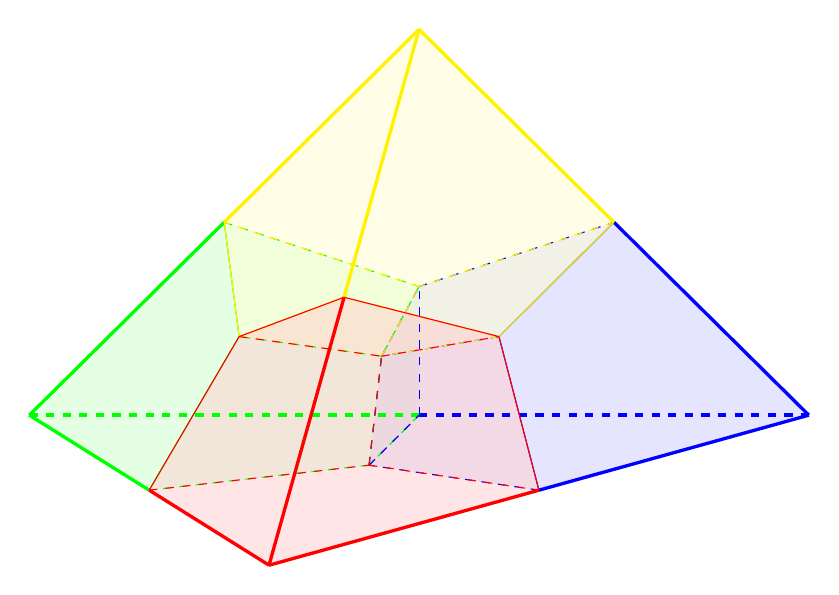
\begin{tikzpicture}[scale=7,rotate around x=270,rotate around z=45]
		%\draw[very thick] (0,0,0) -- (1,0,0) -- (0.5,0.5,0.7) -- (0,1,0) -- cycle;
		%\draw[very thick] (0,0,0) -- (0.5,0.5,0.7);
		%\draw[dashed,very thick] (1,0,0) -- (0,1,0);
		
		\fill[green!20,opacity=0.5] (0,1,0) -- (0,0.5,0) -- (0.3333,0.3333,0) -- (0.5,0.5,0) -- (0.5,0.5,0.2333) -- (0.25,0.75,0.35) -- cycle;
		
		\fill[blue!20,opacity=0.5] (1,0,0) -- (0.5,0,0) -- (0.3333,0.3333,0) -- (0.375,0.375,0.175) -- (0.5,0.5,0.2333) -- (0.75,0.25,0.35) -- cycle;
		
		\fill[yellow!20,opacity=0.5] (0.5,0.5,0.7) -- (0.75,0.25,0.35) -- (0.5,0.1666,0.2333) -- (0.375,0.375,0.175) -- (0.1666,0.5,0.2333) -- (0.25,0.75,0.35) -- cycle;

		\fill[red!20,opacity=0.5] (0,0,0) -- (0,0.5,0) -- (0.1666,0.5,0.2333) -- (0.25,0.25,0.35) -- (0.5,0.1666,0.2333) -- (0.5,0,0) -- cycle;
		
		\draw[green,dashed,very thick] (0,1,0) -- (0.5,0.5,0);
		\draw[green,dashed] (0.5,0.5,0) -- (0.3333,0.3333,0);
		\draw[green,dashed] (0.3333,0.3333,0) -- (0,0.5,0);
		\draw[green,very thick] (0,0.5,0) -- (0,1,0);
		\draw[green,dashed] (0.25,0.75,0.35) -- (0.5,0.5,0.2333);
		\draw[green,dashed] (0.5,0.5,0.2333) -- (0.375,0.375,0.175);
		\draw[green,dashed] (0.375,0.375,0.175) -- (0.1666,0.5,0.2333);
		\draw[green] (0.1666,0.5,0.2333) -- (0.25,0.75,0.35);
		\draw[green,very thick] (0,1,0) -- (0.25,0.75,0.35);
		\draw[green,dashed] (0.5,0.5,0) -- (0.5,0.5,0.2333);
		\draw[green,dashed] (0.3333,0.3333,0) -- (0.375,0.375,0.175);
		\draw[green] (0,0.5,0) -- (0.1666,0.5,0.2333);
		
		\draw[blue,very thick] (1,0,0) -- (0.5,0,0);
		\draw[blue,dashed] (0.5,0,0) -- (0.3333,0.3333,0);
		\draw[blue,dashed] (0.3333,0.3333,0) -- (0.5,0.5,0);
		\draw[blue,dashed,very thick] (0.5,0.5,0) -- (1,0,0);
		\draw[blue] (0.75,0.25,0.35) -- (0.5,0.1666,0.2333);
		\draw[blue,dashed] (0.5,0.1666,0.2333) -- (0.375,0.375,0.175);
		\draw[blue,dashed] (0.375,0.375,0.175) -- (0.5,0.5,0.2333);
		\draw[blue,dashed] (0.5,0.5,0.2333) -- (0.75,0.25,0.35);
		\draw[blue,very thick] (1,0,0) -- (0.75,0.25,0.35);
		\draw[blue] (0.5,0,0) -- (0.5,0.1666,0.2333);
		\draw[blue,dashed] (0.3333,0.3333,0) -- (0.375,0.375,0.175);
		\draw[blue,dashed] (0.5,0.5,0) -- (0.5,0.5,0.2333);
		
		\draw[yellow,very thick] (0.5,0.5,0.7) -- (0.25,0.25,0.35);
		\draw[yellow] (0.25,0.25,0.35) -- (0.5,0.1666,0.2333);
		\draw[yellow] (0.5,0.1666,0.2333) -- (0.75,0.25,0.35);
		\draw[yellow,very thick] (0.75,0.25,0.35) -- (0.5,0.5,0.7);
		\draw[yellow] (0.25,0.75,0.35) -- (0.1666,0.5,0.2333);
		\draw[yellow,dashed] (0.1666,0.5,0.2333) -- (0.375,0.375,0.175);
		\draw[yellow,dashed] (0.375,0.375,0.175) -- (0.5,0.5,0.2333);
		\draw[yellow,dashed] (0.5,0.5,0.2333) -- (0.25,0.75,0.35);
		\draw[yellow,very thick] (0.5,0.5,0.7) -- (0.25,0.75,0.35);
		\draw[yellow] (0.25,0.25,0.35) -- (0.1666,0.5,0.2333);
		\draw[yellow,dashed] (0.5,0.1666,0.2333) -- (0.375,0.375,0.175);
		\draw[yellow,dashed] (0.75,0.25,0.35) -- (0.5,0.5,0.2333);

		\draw[red,very thick] (0,0,0) -- (0,0.5,0);
		\draw[red,dashed] (0,0.5,0) -- (0.3333,0.3333,0);
		\draw[red,dashed] (0.3333,0.3333,0) -- (0.5,0,0);
		\draw[red,very thick] (0.5,0,0) -- (0,0,0);
		\draw[red] (0.25,0.25,0.35) -- (0.1666,0.5,0.2333);
		\draw[red,dashed] (0.1666,0.5,0.2333) -- (0.375,0.375,0.175);
		\draw[red,dashed] (0.375,0.375,0.175) -- (0.5,0.1666,0.2333);
		\draw[red] (0.5,0.1666,0.2333) -- (0.25,0.25,0.35);
		\draw[red,very thick] (0,0,0) -- (0.25,0.25,0.35);
		\draw[red] (0,0.5,0) -- (0.1666,0.5,0.2333);
		\draw[red,dashed] (0.3333,0.3333,0) -- (0.375,0.375,0.175);
		\draw[red] (0.5,0,0) -- (0.5,0.1666,0.2333);
		
		% centre : (0.375,0.375,0.175)
		% face 1 : (0.3333,0.3333,0)
		% face 2 : (0.5,0.1666,0.2333)
		% face 3 : (0.5,0.5,0.2333)
		% face 4 : (0.1666,0.5,0.2333)
		% edge 1 : (0.5,0,0)
		% edge 2 : (0.5,0.5,0)
		% edge 3 : (0,0.5,0)
		% edge 4 : (0.25,0.25,0.35)
		% edge 5 : (0.75,0.25,0.35)
		% edge 6 : (0.25,0.75,0.35)
		
		
		
		%\draw[very thick] (0,0,0) -- (1,0,0) -- (0,1,0) -- cycle;
		%\draw[blue] (0,0,0) -- (0.5,0.5,0.7);
		%\draw[red] (1,0,0) -- (0.5,0.5,0.7);
		%\draw[green] (0,1,0) -- (0.5,0.5,0.7);
		\end{tikzpicture}
	\end{center}
\end{figure}


Les kernels de calcul sont alors appliqués zone par zone dans l'ordre suivant
pour déterminer la dérivée en temps du champ électromagnétique :
\begin{itemize}
	\item terme de volume (\ref{ssect:terme_de_rigidite}) ;
	\item terme de flux (\ref{ssect:terme_de_flux}) ;
	\item terme de masse (\ref{ssect:terme_de_masse}).
\end{itemize}
Dans la plupart des schémas temporels, la mise-à-jour des champs est effectuée
avec une étape de type Euler.
Le graphe des tâches du schéma couplé GD-RK$2$ est donné dans la figure \ref{img:graphe_rk2}.
\\


\begin{figure}[!h]
	\centering
	\caption{
		\label{img:graphe_rk2}
		Graphe des tâches d'un demi pas de temps du schéma couplé GD-RK$2$
		pour deux zones homogènes.
	}
	\begin{tikzpicture}[scale=1]
		\node[ellipse,very thick,draw,align=center] (debut)
			at (0,0) {Début du demi\\pas de temps};

		\node[ellipse,very thick,draw=blue,fill=blue!10,align=center] (volume1)
			at (-4.5,-4) {Zone 1\\Terme de volume};
		\node[ellipse,very thick,draw=red,fill=red!10,align=center] (flux1)
			at (-4,-8) {Zone 1\\Terme de flux};
		\node[ellipse,very thick,draw=green,fill=green!10,align=center] (masse1)
			at (-3,-10) {Zone 1\\Terme de masse};
		\node[ellipse,very thick,draw=gray,fill=gray!10,align=center] (euler1)
			at (-2.5,-12) {Zone 1\\Etape d'Euler};

		\node[ellipse,very thick,draw=blue,fill=blue!10,align=center] (volume2)
			at (4.5,-4) {Zone 2\\Terme de volume};
		\node[ellipse,very thick,draw=red,fill=red!10,align=center] (flux2)
			at (4,-8) {Zone 2\\Terme de flux};
		\node[ellipse,very thick,draw=green,fill=green!10,align=center] (masse2)
			at (3,-10) {Zone 2\\Terme de masse};
		\node[ellipse,very thick,draw=gray,fill=gray!10,align=center] (euler2)
			at (2.5,-12) {Zone 2\\Etape d'Euler};

		\node[rectangle,very thick,draw=red,fill=red!10,align=center] (extract1)
			at (-2,-2) {Interface\\Zone 1\\Extrapolation};
		\node[rectangle,very thick,draw=red,fill=red!10,align=center] (apply1)
			at (-2,-6) {Interface\\Zone 1\\Application du flux};
			
		\node[rectangle,very thick,draw=red,fill=red!10,align=center] (itfflux)
			at (0,-4) {Interface\\Calcul du flux};
		
		\node[rectangle,very thick,draw=red,fill=red!10,align=center] (extract2)
			at (2,-2) {Interface\\Zone 2\\Extrapolation};
		\node[rectangle,very thick,draw=red,fill=red!10,align=center] (apply2)
			at (2,-6) {Interface\\Zone 2\\Application du flux};
		
		\node[ellipse,very thick,draw,align=center] (fin)
			at (0,-14) {Fin du demi\\pas de temps};
			
		\path[arrows={-latex},very thick] (debut) edge[out=180,in=90] (volume1);
		\path[arrows={-latex},very thick] (debut) edge[out=0,in=90] (volume2);
		\path[arrows={-latex},very thick] (volume1) edge (flux1);
		\path[arrows={-latex},very thick] (volume2) edge (flux2);
		\path[arrows={-latex},very thick] (flux1) edge (masse1);
		\path[arrows={-latex},very thick] (flux2) edge (masse2);
		\path[arrows={-latex},very thick] (masse1) edge (euler1);
		\path[arrows={-latex},very thick] (masse2) edge (euler2);
		\path[arrows={-latex},very thick] (euler1) edge (fin);
		\path[arrows={-latex},very thick] (euler2) edge (fin);
		
		\path[arrows={-latex},very thick] (debut) edge[out=195,in=90] (extract1);
		\path[arrows={-latex},very thick] (debut) edge[out=345,in=90] (extract2);
		\path[arrows={-latex},very thick] (extract1) edge (itfflux);
		\path[arrows={-latex},very thick] (extract2) edge (itfflux);
		\path[arrows={-latex},very thick] (itfflux) edge (apply1);
		\path[arrows={-latex},very thick] (itfflux) edge (apply2);
		\path[arrows={-latex},very thick] (apply1) edge[out=290,in=40] (masse1);
		\path[arrows={-latex},very thick] (apply2) edge[out=250,in=140] (masse2);
	\end{tikzpicture}
\end{figure}




\subsection{Etape de type Euler}
\label{ssect:etape_euler}

La mise-à-jour des champs est effectuée avec une étape de type Euler dont
la parallélisation est aisée. En effet, chaque valeur du tableau des dérivées
en temps est utilisée pour mettre à jour la valeur du champ située à la même
position dans un autre tableau ordonné à l'identique.

Ce kernel (figure \ref{img:kernel_euler}) n’utilise aucune donnée géométrique
ou d’interpolation, nous pouvons donc associer un work-item à chaque composante
du champ sans tenir compte de la répartition en zones. Ainsi, chacun effectue
le calcul pour la composante qui lui est associée.

Enfin, les lectures et écritures en mémoire sont coalescentes dans ce cas et
l'utilisation de la mémoire locale s'avère inutile puisque aucun calcul
intermédiaire n'est effectué.
\\

\begin{figure}[h]
	\begin{center}
		\caption{
			\label{img:kernel_euler}
			Kernel de calcul de l’étape Euler.
		}

		\begin{lstlisting}
__kernel void euler(double dt,
                    __global const double* Wn,
                    __global const double* dtWn,
                    __global double* Wnp1) {
    // Numero du work-item
    const int i = get_global_id(0);
    
    // Mise a jour
    Wnp1[i] = Wn[i] + dt * dtWn[i];
}
		\end{lstlisting}
	\end{center}
\end{figure}



\subsection{Kernel du terme de masse}
\label{ssect:kernel_masse}


L’intégrale \eqref{eq:terme_de_masse} qui représente le terme de masse
est calculée par un kernel parallélisé sur un nombre de work-items égal au nombre
de points d'approximation présents dans le maillage.
Les points d'approximation d'une même maille sont regroupés dans un work-group.
Nous notons $\WGId \in \Range{0}{\NE - 1}$ le numéro du
work-group courant et $\WIId \in \Range{0}{\VNPG - 1}$ le numéro
du work-item courant dans son work-group.


Dans un premier temps, chaque work-item lit en mémoire globale les coordonnées
des nœuds de la maille à laquelle il est associé. Ensuite, chaque work-item calcule
le poids d'intégration $\GLW{\WIId}$ de la fonction de base $\PsiRef{\WIId}$
associée au point d'approximation $\GLN{\WIId}$ et le jacobien de la
transformation géométrique en ce même point.
Enfin, la dérivée en temps des champs au point d'approximation $\GLN{\WIId}$
est mise-à-jour en mémoire globale en la divisant par le produit
$\GLW{\WIId} \Jac{\TGeo{\L}} (\GLN{\WIId})$.

Dans ce kernel, le regroupement des work-items par maille est uniquement utilisé
pour récupérer les nœuds de la maille.
\\




\subsection{Kernel du terme de volume}
\label{ssect:kernel_volume}


L’intégrale \eqref{eq:terme_de_rigidite} qui représente le terme de volume
est calculée par un kernel parallélisé sur un nombre de work-items égal au
nombre de fonctions de base définies sur la zone considérée.
Les fonctions de base à support sur une même maille sont regroupées dans un
work-group.
Cette répartition est équivalente à celle utilisée pour le terme de masse.
Nous notons $\WGId \in \Range{0}{\NE - 1}$ le numéro du
work-group courant et $\WIId \in \Range{0}{\VNPG - 1}$ le numéro
du work-item courant dans son work-group.


Dans un premier temps, chaque work-item lit en mémoire globale les coordonnées
des nœuds de la maille à laquelle il est associé. Cette étape est nécessaire
et requiert plusieurs lectures en mémoire non coalescentes car le maillage
est généralement non structuré. Ensuite, les champs de la maille
$\WGId$ sont lus et stockés en mémoire locale. Cette lecture est faite de manière parallèle : chaque work-item lit les champs du point d'approximation qui lui
est associé. La coalescence des données lues est assurée par l'ordre de
stockage des champs illustré par la figure \ref{img:stockage_coalescent}.
Après le chargement des champs en mémoire locale, une synchronisation
locale est nécessaire.


Nous calculons alors l’intégrale \eqref{eq:terme_de_rigidite} sur les mailles hexaédriques
en tirant parti de la
propriété vérifiée par le gradient des fonctions de base exposée dans la section
\ref{ssect:terme_de_rigidite}. Pour un work-item d'indice
$\WIId$, nous évaluons cette intégrale en ne considérant que les points alignés
avec le point d'indice $\WIId$. Observons alors les termes de cette somme :
\begin{align}
	\sum_{j} \GLW{j}
		\Flux{\W_{\L,j}}{\W_{\L,j}}{\Com{\TGeo{\L}'}
		\hat{\nabla} \PsiRef{i}(\GLN{j})} .
\end{align}


Les termes demandant le plus de calcul sont le flux $\F$ et la comatrice
$\Com{\TGeo{\L}'}$. Le flux dépend des deux indices $i$ et $j$,
alors que la comatrice ne dépend que de l’indice $j$. Nous pouvons aussi
rappeler que le gradient $\hat{\nabla} \PsiRef{i}$ s'annule en tout point
d'approximation non aligné avec $\GLN{j}$.
Nous parallélisons ce calcul en attribuant à un work-item le calcul des
termes pour un indice $i$ fixé (fonctions de base) afin d'éviter les écritures concurrentes qu'il
faudrait gérer en parallélisant par rapport à l'indice $j$ (points d'approximation).
Pour cela, nous considérons le multi-indice $\VMId{p}$ tel que
$\WIId = \VMIdToId{p}$. Les indices des poins alignés avec $\GLN{\WIId}$
dans une direction sont obtenus en faisant varier la composante du multi-indice
de cette direction.

Soit $R_\Deg$ l’application qui à un entier associe le reste de la division
euclidienne de cet entier par $\Deg + 1$.
Nous pouvons alors définir les $3$ fonctions d'indices :
\begin{equation}
	\begin{aligned}
		\WIId_0(\alpha) &=
			R_\Deg(\MId{p}{0} + \alpha) +
			(\Deg + 1) (\MId{p}{1} + (\Deg + 1) \MId{p}{2}) , \\
		\WIId_1(\alpha) &=
			\MId{p}{0} + (\Deg + 1) (R_\Deg(\MId{p}{1} + \alpha) +
			(\Deg + 1) \MId{p}{2}) , \\
		\WIId_2(\alpha) &=
			\MId{p}{0} + (\Deg + 1) (\MId{p}{1} +
			(\Deg + 1) R_\Deg(\MId{p}{2} + \alpha)) .
	\end{aligned}
\end{equation}
pour $\alpha$ variant dans l'intervalle $\RangeDeg$.

Chaque work-item (fonction de base) ajoute les contributions qu’il calcule à un tableau privé
contenant la dérivée en temps au point d'approximation associé.
Enfin, la dérivée en temps est mise-à-jour en mémoire globale par des accès coalescents.

Le calcul du terme de volume est très bien adapté à la parallélisation 
et l’algorithme décrit ci-dessus est donné en pseudo-code dans la figure
\ref{img:kernel_volume}.


\begin{figure}[!h]
	\begin{center}
		\caption{
			\label{img:kernel_volume}
			Algorithme parallèle du calcul du terme de volume.
		}
		
		\begin{lstlisting}
iel // indice du work-group (de l'element)
i // indice du work-item (de la fonction de base)
S // sommets de l'element

// Copie des champs de l'element en memoire locale
local_Wn[i] = global_Wn[iel][i]

Synchronisation_locale

// Initialisation de la derivee des champs
dtWn = 0

for (dir = 0; dir < 3; ++dir) { // directions
  for (a = 0; a < d + 1; ++a) { // alignement
    // Calcul de l'indice j
    j = i_dir(a)
    
    // Donnees d'interpolation (utilise S)
    g_j // point d'integration j
    w_j // poids d'integration j
    
    // Calcul de la comatrice
    // de la transformation (utilise S et g_j)
    codtau = comatrice au point j
    
    // Calcul du gradient
    gradpsi = gradient i au point j
    
    // Ajout des contributions en memoire locale
    dtWn += w_j *
        F(local_Wn[j], local_Wn[j], codtau * gradpsi)
  }
}

// Mise a jour en memoire globale
global_dtWn[iel][i] += dtWn
		\end{lstlisting}
	\end{center}
\end{figure}


\begin{remark}
	Les champs en mémoire globale sont stockés de façon à ce que les
	accès soient coalescents. Ce rangement des données est nécessaire 
	afin d'assurer l'efficacité des lectures et écritures.
\end{remark}

\begin{remark}
	L’utilisation de la mémoire locale est impérative. Dans le
	cas contraire, un grand nombre d’accès non coalescents à la mémoire globale
	seraient effectués, dégradant fortement les performances.
\end{remark}

\begin{remark}
	Le chargement en mémoire locale s'effectue en parallèle :
	chaque work-item charge les champs qui lui sont associés.
	Après le chargement en mémoire locale, les work-items sont
	synchronisés, ce qui assure que toutes les données utiles pour la
	suite du calcul sont disponibles.
\end{remark}

\begin{remark}
	Au cours de la boucle sur les points j, nous ne calculons pas toutes
	les composantes du gradient de la fonction de base. En effet,
	puisque i est différent de j, seule la composante correspondant à la direction
	d’alignement de i et j est non nulle.
\end{remark}

\begin{remark}
	Dans le cas des mailles non hexaédriques, la propriété de nullité du gradient
	des fonctions de base ne s'applique pas et tous les termes de la somme
	approximant le terme de volume doivent être calculés dans les $3$ directions
	de l'élément de référence.
	\\
\end{remark}



\subsection{Kernels du terme de flux}
\label{ssect:kernel_surface}

Le terme de flux représente les échanges aux interfaces entre les
mailles d'une même zone homogène. Le raccord entre ces mailles
est conforme et leurs ordres d'interpolation sont identiques.

Rappelons la formule d'approximation du terme de flux entre deux
mailles homogènes \eqref{eq:terme_de_flux} :
\begin{align}
	\GLW{f,\pi(f,i)} \PsiRef{i}(\GLN{f,\pi(f,i)})
	\Flux{\W_{\L,f,\pi(f,i)}}
		{\W_{\R,f',\GLNFPermut(\pi(f,i))}}
		{\Com{\TGeo{\L}'} \hat{\n}} .
\end{align}
Cette intégrale est calculée en trois étapes. 
La première étape consiste en l'extrapolation des champs du volume sur les faces de chaque maille.
Ensuite, les flux sont calculés à partir des champs extraits dans la seconde étape,
puis appliqués à la dérivée en temps dans la dernière étape.
Chacune de ces étapes est effectuée par un kernel distinct.


\subsubsection{Extrapolation des champs}
\label{sssect:kernel_surface_extraction}

L'extrapolation est parallélisée sur un nombre de work-groups égal au nombre de mailles
présentes dans la zone considérée. Chaque work-group est composé d'autant de
work-items qu'il y a de points d'approximation sur les faces d'une maille.
Nous notons $\WGId \in \Range{0}{\NE - 1}$ le numéro du
work-group courant et $\WIId_b$ le numéro du work-item courant dans son work-group. L'indice de la face $f \in \Range{0}{5}$ associé à chaque
work-item ainsi que l'indice du point d'approximation $\WIId_f \in \Range{0}{\SNPG - 1}$
sur cette face sont calculés à partir de l’indice $\WIId_b$ du work-item tels que :
\begin{align} \label{eq:kernel_decomp_face_id}
	\WIId_b = \WIId_f + f \SNPG .
\end{align}

Dans un premier temps, les work-items se partagent la lecture en mémoire
globale des champs de la maille
$\WGId$ et les stockent en mémoire locale.
Cette étape est effectuée comme
dans le calcul des termes de volume, par les
$\VNPG$ premiers work-items.

\begin{remark} \label{rq:kernel_flux_delta_pg_1}
	Jusqu'à l'ordre d'interpolation $5$ y compris,
	le nombre de points de faces d'une maille est supérieur (ou égal)
	au nombre de points volumiques. En effet, lorsque $\Deg=5$,
	$6 \SNPG = \VNPG$. Au-dessous, certains work-items restent
	inactifs au cours de cette étape. Au-delà, certaines données
	ne sont pas chargées en mémoire locale, mais en pratique nous
	n'utilisons jamais d'interpolation d'ordre supérieur à $5$.
\end{remark}

Chaque work-item calcule alors la valeur des champs provenant de la maille
sur le point de face qui lui est associé.
Pour cela nous commençons par calculer les coordonnées du point de face $\WIId_b$ dans
l’élément de référence. Ensuite, nous ajoutons les contributions des fonctions de base
en ce point.
Dans notre cas de mailles hexaédriques, seules les fonctions de base associées aux points
d'approximation alignés avec le point de face considéré sont non nulles en ce point
(proposition \ref{prop:projection_face}). Ainsi, seules $\Deg + 1$ contributions
sont à prendre en compte, contre celles de toutes les fonctions
de base de la maille dans le cas non hexaédrique.

Ces champs extrapolés sont ensuite stockés de façon coalescente
en mémoire globale à destination du kernel chargé de calculer le flux.
L’algorithme décrit ci-dessus est donné en pseudo-code dans la figure
\ref{img:kernel_surface_extract}.



\begin{figure}[!h]
	\begin{center}
		\caption{
			\label{img:kernel_surface_extract}
			Algorithme parallèle de l'extrapolation des champs
			dans le calcul du terme de flux.
		}
		
		\begin{lstlisting}
iel // indice du work-group (de l'element)
ib // indice du work-item (du point de bord)

f = ib / (d + 1)^2 // indice de face
i = ib % (d + 1)^2 // indice du point sur la face

// Copie des champs de l'element en memoire locale
if (ib < (d + 1)^3)
  local_Wn[ib] = global_Wn[iel][ib]

Synchronisation_locale

// Calcul des coordonnees du point de reference
g^_{f,i} // point i sur face f

// Initialisation de la valeur des champs
face_Wn = 0

dir // direction normale a la face f
for (a = 0; a < d + 1; ++a) { // alignement
  // Calcul de l'indice de la fonction de base
  j = i_dir(a)

  // Extrapolation
  face_Wn += psi_j(g^_{f,i}) * local_Wn[j]
}

// Stockage en memoire globale
global_face_Wn[iel][ib] = face_Wn
		\end{lstlisting}
	\end{center}
\end{figure}


\subsubsection{Calcul des flux}
\label{sssect:kernel_surface_flux}

Le calcul des flux est parallélisé de la même façon que l'extrapolation
des champs : un nombre de work-groups égal au nombre de mailles
présentes dans la zone considérée et autant de
work-items qu'il y a de points d'approximation sur les faces d'une maille.
Nous notons $\WGId$ le numéro du
work-group courant et $\WIId_b$ le numéro du work-item courant dans son work-group. L'indice de la face $f$ ainsi que l'indice du point
d'approximation $\WIId_f$ sont calculés comme précédemment
\eqref{eq:kernel_decomp_face_id}.

Dans un premier temps, chaque work-item lit en mémoire globale les coordonnées
des nœuds de la maille à laquelle il est associé.
Comme pour le kernel de volume, cette étape est nécessaire
et requiert plusieurs lectures en mémoire non coalescentes car le maillage
est généralement non structuré.
Les work-items chargent aussi en mémoire locale
les champs extraits dans le kernel d'extrapolation au point de face
associé. Cette lecture est faite en accès coalescent.

Ensuite, lorsque le flux numérique classique s'applique
\eqref{eq:flux_numerique}, en l'absence
de modèle de surface spécifique (chapitre \ref{chap:modeles}),
nous chargeons les champs de face extraits de la maille voisine $\R$.
Pour cela nous calculons l'indice du point de face de la maille $\R$
correspondant au point courant de la maille $\L$ grâce aux données
de connectivité des mailles et en tenant compte des orientations des faces.
Cette lecture est généralement faite en accès non-coalescent, compte tenu
de la structure du maillage.

Pour terminer cette étape, chaque work-item calcule le flux numérique
au point qui lui est associé. Nous devons pour cela calculer les
coordonnées physiques du point d’intégration ainsi que la normale
en ce point.
Les coordonnées physiques ne servent que pour certains flux spécifiques,
mais elles sont nécessaires pour le calcul de la normale.

Ces flux sont ensuite stockés en mémoire globale de façon coalescente
à destination du kernel chargé d'ajouter leur contribution au tableau
de la dérivée temporelle de la solution.
L’algorithme décrit ci-dessus est donné en pseudo-code dans la figure
\ref{img:kernel_surface_flux}.

\begin{figure}[!h]
	\begin{center}
		\caption{
			\label{img:kernel_surface_flux}
			Algorithme parallèle du calcul du flux.
		}
		
		\begin{lstlisting}
iel // indice du work-group (de l'element)
ib // indice du work-item (du point de bord)
S // sommets de l'element
t // temps physique courant

f = ib / (d + 1)^2 // indice de face
i = ib % (d + 1)^2 // indice du point sur la face

// Copie des champs du point de face
WL = global_face_Wn[iel][ib]

// Copie des champs du point de face voisin
jel // indice de la maille voisine
if (jel) {
  jb // indice du point voisin (utilise jel, i et f)
  WR = global_face_Wn[jel][jb]
}

// Donnees d'interpolation (utilise S, i et f)
g_i // point d'integration i
w_i // poids d'integration i
n_i // normale au point i

// Initialisation de la valeur du flux
face_flux = 0

// Calcul du flux (utilise aussi g_i et t en fonction
// du type de flux)
face_flux = F(WL, WR, n_i)

// Stockage en memoire globale
// Application directe du poids d'integration
global_face_flux[iel][ib] = face_flux * w_i
		\end{lstlisting}
	\end{center}
\end{figure}


  



\subsubsection{Application à la dérivée}
\label{sssect:kernel_surface_application}


Ce kernel est parallélisé de la même façon que le kernel de volume :
un nombre de work-groups égal au nombre de mailles
présentes dans la zone considérée et autant de work-items
qu'il y a de fonctions de base définies sur la maille considérée.
Nous notons $\WGId$ le numéro du
work-group courant et $\WIId$ le numéro du work-item courant dans son work-group.

Dans un premier temps, les work-items se partagent la lecture en mémoire
globale des flux calculés sur les faces de la maille
$\WGId$ et les stockent en mémoire locale.
Comme précisé dans la remarque \ref{rq:kernel_flux_delta_pg_1},
le nombre de points de volume (ou de fonctions de base)
est généralement inférieur au nombre de points de faces.
Une boucle optimisée a donc été implémentée afin de charger ces
flux en réduisant l'inactivité de certains work-items :
à chaque itération, $\VNPG$ valeurs sont copiées en accès coalescent.
A l'ordre $0$, $6$ itération sont nécessaires ;
à l'ordre $1$, $3$ itérations sont nécessaires ;
aux ordres $2$ à $4$, $2$ itérations sont nécessaires ;
et aux ordres supérieurs à $5$, une seule itération est nécessaire.
Après le chargement des flux en mémoire locale, une synchronisation
locale doit être effectuée.

Ensuite, chaque work-item $\WIId$ calcule l’intégrale
\eqref{eq:terme_de_flux} pour chaque face de la maille.
En appliquant la propriété \ref{prop:projection_face},
ce calcul ne nécessite que la contribution d’un flux par face :
pour une face $f$ donnée, le seul flux utilisé est celui associé au point
de face sur lequel le point de volume est projeté.
Chaque work-item (fonction de base) ajoute les contributions qu’il calcule à un tableau privé
contenant la dérivée en temps au point d'approximation associé.

Enfin, la dérivée en temps est mise-à-jour en mémoire globale par des accès coalescents.
L’algorithme décrit ci-dessus est donné en pseudo-code dans la figure
\ref{img:kernel_surface_apply}.
\\

\begin{figure}[!h]
	\begin{center}
		\caption{
			\label{img:kernel_surface_apply}
			Algorithme parallèle de l'application des flux
			à la dérivée temporelle.
		}
		
		\begin{lstlisting}
iel // indice du work-group (de l'element)
i // indice du work-item (de la fonction de base)

// Copie des flux ponderes en memoire locale
// Boucle optimisee
j_max = ceil(6 * (d + 1)^2 / (d + 1)^3)
for (j = 0; j < j_max; ++j) {
  ib = i + j * (d + 1)^3 // point de face
  if (ib < 6 * (d + 1)^2)
    face_flux[ib] = global_face_flux[iel][ib]
}

Synchronisation_locale

// Initialisation de la derivee des champs
dtWn = 0

for (f = 0; f < 6; ++f) { // faces
  j // indice du point de face aligne
  jb = j + f * (d + 1)^2 // indice du point de bord

  // Calcul des coordonnees du point de reference
  g^_{f,j} // point j sur face f

  // Application du flux pondere
  dtWn -= psi_i(g^_{f,j}) * face_flux[jb]
}

// Mise a jour en memoire globale
global_dtWn[iel][i] += dtWn
		\end{lstlisting}
	\end{center}
\end{figure}




\subsection{Kernels du terme d'interface}
\label{ssect:kernel_interface}


Le terme d'interface représente les échanges entre les
mailles de $2$ zones homogènes distinctes. Le raccord entre ces mailles
n'est pas nécessairement conforme ou leurs ordres d'interpolation sont
distincts. Dans ce cas, les points d'interpolation des faces
ne coïncident pas.

Nous identifions alors le côté le plus finement discrétisé spatialement
\ref{rq:kernel_interface_choix}, supposons qu'il s'agit du côté gauche.
Les points d'interpolation de face des mailles de gauche situés
sur l'interface servent de points d'extrapolation des champs.
Ainsi, sur une maille $\L$ du côté gauche,
le comportement des kernels est identique
à un simple terme de flux homogène (section \ref{ssect:kernel_surface}).

Du côté droit, sur une maille $\R$,
puisque les points d'extrapolation (ou d'interface)
ne sont pas les projetés des points de volume, l'extrapolation
et l'application des flux ne bénéficient pas des simplifications
apportées par les propriétés des fonctions de base.
Ainsi, l'extrapolation des champs sur les points d'interface
nécessite de calculer la somme complète \eqref{eq:extract_complete}
pour les $\VNPG$ fonctions de base (contre $\Deg+1$ dans le cas conforme).
Les coordonnées des points d'interface dans l'élément de référence
associé à la maille $\R$ doivent être calculées
en approchant la réciproque de la transformation
$\TGeo{\R}$ par la méthode de Newton, appliquée
au point d'interface physique.
De plus, le flux calculé en chaque point d'interface de la maille
$\R$ doit ajouter sa contribution à la dérivée temporelle
pour les $\VNPG$ fonctions de base (là encore contre $\Deg+1$
dans le cas conforme).

\begin{remark} \label{rq:kernel_interface_choix}
	En pratique, nous utilisons des maillages à connectivité conforme et
	n'avons que $2$ cas de figure à traiter dans le solveur :
	\begin{itemize}
		\item raccord de face conforme et ordre d'interpolation distinct ;
		\item raccord $1/6$ en bord de domaine (figure \ref{img:raccord_1_6}).
	\end{itemize}
	
	Dans le premier cas, nous extrapolons les champs sur les points
	de face du côté d'ordre le plus élevé. Ce choix est stratégiquement
	le meilleur dans le but de diminuer la quantité de calculs et d'améliorer la précision.
	En effet, nous bénéficions ainsi des simplifications liées
	aux propriétés des fonctions de base du côté le plus coûteux.
	
	Le second cas se présente lors de l'ajout de couches PML
	(section \ref{ssect:PML}) autour d'un maillage en tétraèdres découpés (figure \ref{img:tetra_hexa}).
	Nous obtenons alors un raccord d'une face contre $6$ à cette interface.
	Nous extrapolons alors les champs sur les points de face du côté le
	plus raffiné : le côté interne, non PML.
	\\
\end{remark}


\begin{figure}[h]
	\begin{center}
		\caption{
			\label{img:raccord_1_6}
			Schéma représentant le raccord $1/6$ entre les couches
			de PML adjointes et le maillage initial en tétraèdres découpés (figure \ref{img:tetra_hexa}).
			Les faces des tétraèdres découpés sont représentées en bleu
			et en rouge.
		}
		
		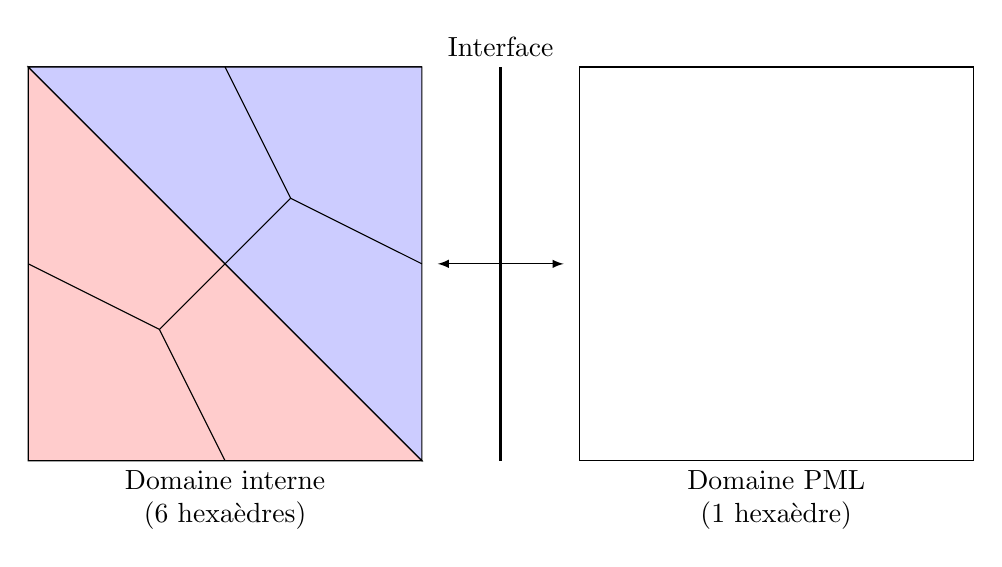
\begin{tikzpicture}[scale=1]
		\draw (0,0) rectangle (5,5);
		\draw[very thick] (6,0) -- (6,5) node[above] {Interface};
		\draw (7,0) rectangle (12,5);
		\draw[arrows={-latex}] (6,2.5) -- (5.2,2.5);
		\draw[arrows={-latex}] (6,2.5) -- (6.8,2.5);
		
		\draw[fill=red!20] (0,0) -- (5,0) -- (0,5) -- cycle;
		\draw[fill=blue!20] (5,0) -- (0,5) -- (5,5) -- cycle;
		
		\draw[-] (2.5,2.5) -- (1.6666,1.6666);
		\draw[-] (2.5,0) -- (1.6666,1.6666);
		\draw[-] (0,2.5) -- (1.6666,1.6666);
		
		\draw[-] (2.5,2.5) -- (3.3333,3.3333);
		\draw[-] (2.5,5) -- (3.3333,3.3333);
		\draw[-] (5,2.5) -- (3.3333,3.3333);
		
		\draw (2.5,0) node[below,align=center] {Domaine interne\\($6$ hexaèdres)};
		\draw (9.5,0) node[below,align=center] {Domaine PML\\($1$ hexaèdre)};
		\end{tikzpicture}
	\end{center}
\end{figure}


\subsection{Parallélisation MPI}
\label{ssect:parallelisation_mpi}

L'architecture classique des (super)calculateurs
possédant des GPU est d'associer un GPU à chaque nœud de calcul. Dans le cas
des CPU (section \ref{sect:adaptation_cpu}), chaque périphérique est par nature un nœud de calcul.
Chaque nœud de calcul possède son propre espace mémoire.
Ainsi, afin de paralléliser les calculs sur plusieurs périphériques OpenCL,
nous utilisons une bibliothèque MPI \cite{10.1007/978-3-0348-8534-8_21}.
Celle-ci permet de réaliser des calculs sur
des machines à mémoire distribuée.
Plusieurs processus sont lancés en parallèle. Chaque processus possède son propre
espace mémoire. Les différents processus communiquent alors entre eux par un système
de messages.

%\todo{PH: in french on dit "bibliothèque"}
Cette bibliothèque permet aussi d'effectuer des calculs sur une machine à mémoire
partagée. Par exemple, les machines de calcul possédées par AxesSim qui associent
plusieurs GPU à un unique nœud de calcul.
Dans ce cas, la mémoire de la machine doit être suffisament grande pour accueillir
tous les processus, car, même si ces derniers sont hébergés dans le même espace
mémoire, chacun gère sa propre copie de la mémoire allouée par le programme
au cours du pré-traitement.
\\ 


Pour paralléliser les calculs sur plusieurs périphériques, le maillage global
est réparti de manière équilibrée entre les différents processus MPI.
Cette subdivision du maillage est effectuée à l'aide de la bibliothèque de
partitionnement \texttt{metis} \cite{Karypis:1998:FHQ:305219.305248}.
Chaque processus utilise un périphérique OpenCL différent pour effectuer
les calculs sur le sous-domaine qui lui a été associé.

Les communications sont effectuées aux interfaces entre les sous-domaines, lors
du calcul du terme de flux. Une telle interface est appelée « interface MPI ».
Le calcul du flux nécessite la connaissance des champs
provenant des mailles voisines. Si la maille voisine est traitée par un processus
différent, l'information doit être récupérée au préalable.

Pour réduire le volume des données communiquées, chaque processus
effectue l'extrapolation des champs de son côté de l'interface MPI. Ceci permet
de diviser le nombre de données échangées par $\Deg + 1$ contrairement à
une méthode qui consisterait à échanger les données volumiques des mailles
voisines de l'interface.
De plus, nous sommes assurés que les données à échanger sont stockées de manière
contiguë dans un unique tableau.

Une fois les champs extraits des deux côtés, les processus partageant une
interface MPI s'échangent ces données afin de calculer le flux.
Cet échange de données est effectué de manière asynchrone à l'aide de threads
dédiés (figure~\ref{img:mpi_interface}). Pour chaque interface MPI et à chaque calcul du terme de flux,
deux threads sont générés (un par processus) : le processus noté $P_0$,
respectivement $P_1$,
transfère les données extraites du périphérique de calcul à l’hôte et les échange
(envoie, réception) avec le processus $P_1$, respectivement $P_0$,
puis transfère les données reçues de l’hôte au périphérique de calcul.
Ensuite, chaque domaine effectue le calcul et l'application du flux.


\begin{figure}[!h]
	\begin{center}
		\caption{
			\label{img:mpi_interface}
			Schéma représentant une interface MPI.
		}
		
		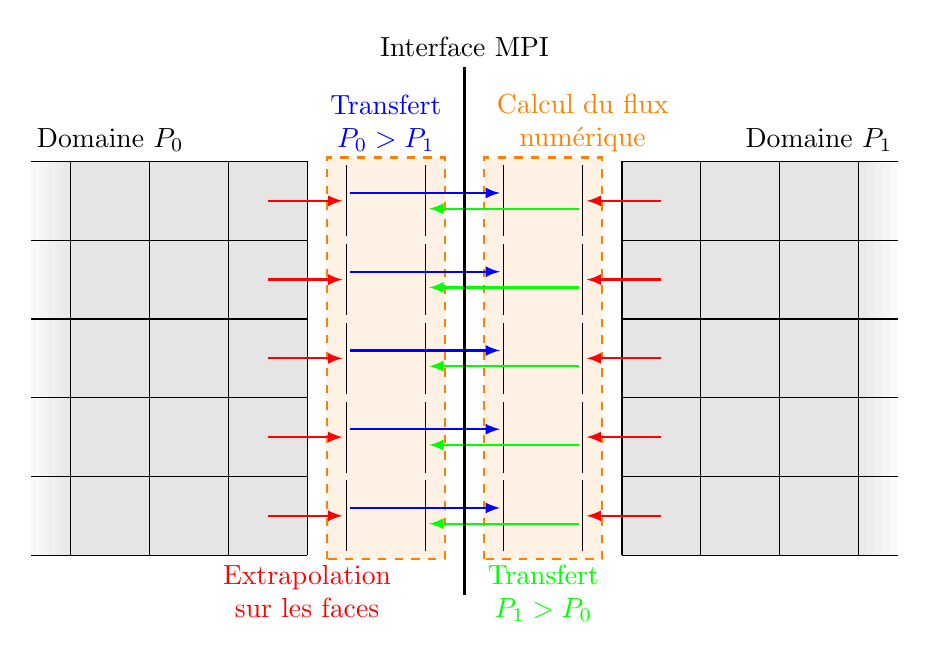
\begin{tikzpicture}[scale=1]
		\draw[thick,dashed,orange,fill=orange!10] (4.25,-0.05) rectangle (5.75,5.05);
		\draw[thick,dashed,orange,fill=orange!10] (6.25,-0.05) rectangle (7.75,5.05);
		
		\fill[gray!20] (1,0) rectangle (4,5);
		\fill[gray!17] (0.9,0) rectangle (1.0,5);
		\fill[gray!14] (0.8,0) rectangle (0.9,5);
		\fill[gray!11] (0.7,0) rectangle (0.8,5);
		\fill[gray!08] (0.6,0) rectangle (0.7,5);
		\fill[gray!05] (0.5,0) rectangle (0.6,5);

		\fill[gray!20] (8,0) rectangle (11,5);
		\fill[gray!17] (11.0,0) rectangle (11.1,5);
		\fill[gray!14] (11.1,0) rectangle (11.2,5);
		\fill[gray!11] (11.2,0) rectangle (11.3,5);
		\fill[gray!08] (11.3,0) rectangle (11.4,5);
		\fill[gray!05] (11.4,0) rectangle (11.5,5);

		\foreach \i in {0,1,2,3,4,5} {
			\draw[-] (0.5,\i) -- (4,\i);
			\draw[-] (8,\i) -- (11.5,\i);
		}
		\foreach \i in {1,2,3,4,8,9,10,11} {
			\draw[-] (\i,0) -- (\i,5);
		}
		\foreach \i in {4.5,5.5,6.5,7.5} {
			\draw[-] (\i,0.05) -- (\i,0.95);
			\draw[-] (\i,1.05) -- (\i,1.95);
			\draw[-] (\i,2.05) -- (\i,2.95);
			\draw[-] (\i,3.05) -- (\i,3.95);
			\draw[-] (\i,4.05) -- (\i,4.95);
		}
		\foreach \i in {0.5,1.5,2.5,3.5,4.5} {
			\draw[arrows={-latex},thick,red] (3.5,\i) -- (4.45,\i);
			\draw[arrows={-latex},thick,red] (8.5,\i) -- (7.55,\i);
		}
		\foreach \i in {0.6,1.6,2.6,3.6,4.6} {
			\draw[arrows={-latex},thick,blue] (4.55,\i) -- (6.45,\i);
		}
		\foreach \i in {0.4,1.4,2.4,3.4,4.4} {
			\draw[arrows={-latex},thick,green] (7.45,\i) -- (5.55,\i);
		}
		
		\draw[very thick] (6,-0.5) -- (6,6.2) node[above] {Interface MPI};
		\draw (1.5,5) node[above] {Domaine $P_0$};
		\draw (10.5,5) node[above] {Domaine $P_1$};
		\draw (4,0) node[below,red,align=center] {Extrapolation\\sur les faces};
		\draw (5,5) node[above,blue,align=center] {Transfert\\$P_0 > P_1$};
		\draw (7,0) node[below,green,align=center] {Transfert\\$P_1 > P_0$};
		\draw (7.5,5) node[above,orange,align=center] {Calcul du flux\\numérique};
		
		\end{tikzpicture}
	\end{center}
\end{figure}


Comme nous l'avons précisé dans la section \ref{ssect:peripheriques_opencl},
la soumission et l'ordonnancement des tâches
sont gérés par un graphe des tâches.
Ce graphe des tâches utilise les évènements de l'API OpenCL pour
contrôler l'ordre des tâches.
Afin d'intégrer un thread de communication MPI dans le graphe des tâches,
son exécution est conditionnée par la complétion d'une liste d'évènements OpenCL (ceux associés aux kernels d'extrapolation)
et un nouvel événement OpenCL est généré à sa soumission. Ce nouvel événement
est marqué comme étant terminé à la fin du thread de communication MPI.
C'est aussi cet évènement qui conditionnera l'exécution du
kernel de calcul du flux d'interface MPI.
\\
%\todo{PH: dernier paragraphe pas très clair}




Le partitionnement du maillage effectué dans le but de diviser le problème
simulé sur plusieurs périphériques de calcul génère des interfaces
supplémentaires qui augmentent le coût de calcul de la simulation.
Ce surcoût diminue l'efficacité du solveur qui doit être étudiée
dans le but de valider l'implémentation MPI.
Nous étudions l'efficacité MPI (ou scalabilité) dans la section
\ref{sect:scalabilite}.
\\


\section{Adaptations CPU}
\label{sect:adaptation_cpu}


Les kernels optimisés pour GPU présentés dans la section
\ref{sect:implementation_gpu} fonctionnent aussi sur CPU mais ne sont
pas optimisés pour ces derniers.
La différence d'architecture --- SIMD pour les GPU \textit{versus}
MIMD pour les CPU --- implique une différence de performances
pour un même kernel.

Les axes d'optimisation sont documentés par les constructeurs
des CPU (Intel \cite{intelsdkguide}, AMD \cite{amdsdkguide}). Afin d'améliorer les performances d'un kernel
sur CPU, les points suivants sont à respecter :
\begin{itemize}
	\item n'utiliser que la mémoire globale ;
	\item augmenter la sérialisation des traitements ;
	\item préférer stocker les résultats récurrents ;
	\item solliciter les unités de calcul vectoriel.
\end{itemize}
Nous présentons dans la suite les gains de performance constatés
suite à l'application de ces différentes étapes \cite{weber:hal-01666352}.
Les accélérations présentées ont été obtenues à l'ordre d'interpolation
spatiale $\Deg=2$.

Le cas d'application utilisé est la propagation d'une onde plane dans une grille régulière
(section \ref{sect:valid_onde_plane}).
Nous procédons à quelques itérations sur un maillage cube de $90$ mailles par côté.
Les périphériques utilisés pour ces résultats sont un
CPU Intel Core i7-920 et un GPU NVidia GeForce GTX 460.
Initialement, ce CPU est $15.97$ fois plus lent que ce GPU
lorsque nous utilisons les mêmes kernels (optimisés pour GPU).
La répartition en temps de calcul des différents kernels GPU est présentée
dans le tableau \ref{tab:comp_cpu_gpu_avant}.

\begin{figure}[!h]
	\begin{center}
		\caption{
			\label{tab:comp_cpu_gpu_avant}
			Comparaison de la répartition en temps de calcul sur CPU Intel Core i7-920 et GPU NVidia GeForce GTX 460 des
			principaux kernels
			de calcul optimisés pour GPU (avant spécialisation pour CPU).
		}
		
		\begin{tabular}{|c|c|c|}
			\hline
			 & GPU & CPU \\ \hline\hline
			Temps total (s) & $17.49$ & $279.38$ \\	\hline
			Volume (\%) & $23.47$ & $47.57$ \\	\hline
			Flux (\%) & $68.75$ & $48.71$ \\	\hline
			Masse (\%) & $5.17$ & $2.58$ \\	\hline
			Euler (\%) & $1.88$ & $0.81$ \\	\hline
		\end{tabular}
	\end{center}
\end{figure}

Etant déjà en possession de kernels optimisés GPU, l'objectif
de ces travaux a été de les optimiser au mieux à destination
des CPU, tout en conservant leur essence.
Cette approche nous a permis d'obtenir de bonnes performances,
tout en limitant le coût de développement.
\\


\subsection{Suppression de l'utilisation de la mémoire locale}
\label{ssect:cpu_suppr_memoire_locale}


Pour les CPU, la mémoire locale est généralement
de nature identique à la mémoire globale, dans les deux cas il s'agit
de la mémoire vive du nœud.
Cette information est donnée par l'identifiant \verb|CL_DEVICE_LOCAL_MEM_TYPE|
dans l'API OpenCL.
Contrairement aux GPU pour lesquels le temps d'accès à la mémoire
locale est bien plus rapide que le temps d'accès à la mémoire globale,
dans le cas du CPU ce temps est identique.

Nous avons modifié les kernels du terme de volume \ref{ssect:kernel_volume}
et de flux \ref{ssect:kernel_surface} afin qu'ils ne chargent plus
les champs de la maille considérée en mémoire locale,
les kernels du terme de masse et l'étape d'Euler n'utilisant pas
la mémoire locale.
Les champs sont alors directement lus en mémoire globale dès
que utilisés dans les calculs.

Puisque la mémoire locale n'est plus utilisée, nous ne renseignons plus
la taille des work-groups à l'exécution de ces kernels.
Ce choix est laissé à l'API OpenCL qui regroupe
les work-groups au mieux en fonction du périphérique cible (comportement par défaut).
Nous retrouvons l'indice de la maille et de la fonction de base à traiter
à l'aide d'une division euclidienne de l'indice global du work-item.

Suite à ces modifications (et d'autres simplifications qui en découlent),
nous avons constaté un facteur d'accélération de $2.39$ pour le kernel
du terme de volume.
\\


\subsection{Sérialisation}
\label{ssect:cpu_serialisation}


L'objectif d'un CPU est la polyvalence. Chaque cœur de calcul fonctionne indépendamment avec ses propres unités d'instruction dans le but
d'exécuter des traitements distincts en parallèle
(c'est le principe du « \textit{multitasking} »).
Il n'est donc pas nécessaire de paralléliser le code à l'échelle de
l'instruction, au contraire, l'augmentation de la sérialisation au sein
d'un kernel accorde plus de liberté aux cœurs de calcul et produit de
meilleures performances.
Cette approche permet aussi de bénéficier de l'effet de cache dans
l'accès aux données.

Nous avons modifié le kernel du terme de volume \ref{ssect:kernel_volume}
afin que chaque work-item traite,
non plus une fonction de base, mais l'ensemble des fonctions de base
d'une maille.
Pour cela il a suffi d'ajouter une boucle sur
les fonctions de base englobant le traitement déjà codé dans
le kernel.
Le nombre de work-items passe donc de $\NE \VNPG$
à $\NE$.


Nous avons aussi modifié les kernels du terme 
de flux \ref{ssect:kernel_surface} afin que chaque work-item traite,
non plus un point de face, mais l'ensemble des points 
d'une face dans le cas des étapes d'extrapolation et de calcul du flux.
L'application des flux a été adaptée comme le kernel de volume.
De plus, les deux premières étapes (extraction des champs
et calcul du flux numérique) ont été regroupées en un seul kernel et
les flux sont calculés une seule fois par interface entre mailles,
contre un calcul de flux de chaque côté de l'interface dans le cas
du kernel optimisé pour GPU.
Le nombre de work-items passe donc de 
$6 \NE \SNPG$ à $3 \NE$,
dans le cas de ce kernel fusionné.
L'exécution d'un seul kernel donne de meilleures performances.
Ce choix revient à supprimer une synchronisation globale des work-items.

Suite à ces modifications,
nous avons constaté un facteur d'accélération de $1.40$ pour le kernel
du terme de volume.
Dans le cas des kernels du terme de flux, la combinaison de la
suppression de l'utilisation de la mémoire locale et de la sérialisation
des traitements a mené à une accélération de $2.24$.
\\


\subsection{Stockage des données récurrentes}
\label{ssect:cpu_stockage_const}

Dans l'implémentation GPU, compte tenu de la lenteur des accès mémoire
par rapport à la vitesse de calcul et de l'espace mémoire limité,
nous avons fait le choix de calculer à chaque itération un certain nombre
de données constantes, propres à chaque maille,
dont notamment : le gradient des fonctions de base qui intervient
dans le flux numérique du terme de volume et la valeur de la normale
aux faces qui intervient dans le flux numérique du terme de flux.

En comparaison, la taille mémoire associée aux CPU d'une machine
de calcul est colossale : généralement de 64 à 256 Go contre
8 à 16 Go de mémoire sur un GPU conçu pour le calcul.
Ces données constantes, récurrentes et propres à chaque maille
sont donc pré-calculées puis passées en argument aux kernels,
comme pour les tableaux des champs, des nœuds, de connectivité, \textit{etc.}.

Suite à ces modifications,
nous avons constaté des facteurs d'accélération de $4.45$ pour le kernel
du terme de volume et $1.3$ pour les kernels du terme de flux
avec une augmentation de la taille mémoire de $57$ \%.
\\



\subsection{Unités de calcul vectoriel}
\label{ssect:cpu_unites_vectorielles}

Une action supplémentaire pour améliorer les performances sur CPU
est l'utilisation des unités de calcul vectoriel SSE (pour « \textit{Streaming SIMD Extensions}) ou AVX (pour « \textit{Advanced Vector Extensions} »)
lorsqu'ils en sont pourvus.
Ce sont des architectures pour lesquelles les registres sont de plus grande taille, pouvant ainsi stocker plusieurs valeurs à traiter en parallèle.
Dans le cas AVX-$512$ (dernière génération, avec registres de $512$ bits), il est possible de traiter simultanément
jusqu'à $16$ opérations de nombres réels en simple précision et $8$ en double précision.
Ces valeurs correspondent aussi au facteur d'accélération théorique
lié à l'utilisation de ces capatités vectorielles du CPU.

Cependant, la complexité algorithmique de la méthode GD rend cette adaptation très difficile.
Pour être pleinement efficace, les données devraient être
ordonnées sous forme de vecteurs en mémoire vive afin que
les kernels puissent directement appliquer le masque du type vectoriel
(par exemple \verb|float4| pour un vecteur de $4$ réels simple précision).
Ensuite, tous les kernels doivent traiter les données sous forme
vectorielle (ou être adaptés pour extraire les données des vecteurs),
ce qui implique de devoir adapter tout le code de calcul
avant de pouvoir valider les développements et constater une
accélération.
\\



\subsection{Bilan du gain de performances}
\label{ssect:cpu_bilan}

Finalement,
nous avons constaté une accélération d'un facteur $5.52$
sur le cas d'application décrit plus haut.
Le GPU NVidia GeForce GTX 460 que nous avons utilisé, avec les kernels optimisés pour GPU,
n'est donc plus que $2.90$ fois plus rapide que le CPU Intel Core i7-920
utilisé avec les kernels optimisés pour CPU.
La répartition en temps de calcul des différents kernels après optimisations est présentée
dans le tableau \ref{tab:comp_cpu_gpu_apres}.


\begin{figure}[!h]
	\begin{center}
		\caption{
			\label{tab:comp_cpu_gpu_apres}
			Comparaison de la répartition en temps de calcul sur CPU Intel Core i7-920 et GPU NVidia GeForce GTX 460 des
			principaux kernels
			de calcul optimisés pour l'architecture cible.
		}
		
		\begin{tabular}{|c|c|c|}
			\hline
			& GPU & CPU \\ \hline\hline
			Temps total (s) & $17.49$ & $50.63$ \\	\hline
			Volume (\%) & $23.47$ & $12.90$ \\	\hline
			Flux (\%) & $68.75$ & $70.94$ \\	\hline
			Masse (\%) & $5.17$ & $9.69$ \\	\hline
			Euler (\%) & $1.88$ & $4.47$ \\	\hline
		\end{tabular}
	\end{center}
\end{figure}


Ces résultats sont dépendants des périphériques utilisés. En effet,
dans le cas d'une comparaison entre un CPU Intel Core i7-5820K et un
GPU NVidia GeForce GTX 1070 sur $100$ itérations du cas d'application
\ref{sect:tete_simplifiee}, le facteur d'accélération constaté sur ce CPU
avec l'utilisation des kernels optimisés CPU n'est que de $2.76$.
De plus, ce GPU reste $10$ fois plus rapide que ce CPU, chacun utilisé
avec les kernels optimisés pour son architecture.
La répartition en temps de calcul des différents kernels pour ces périphériques est présentée
dans le tableau \ref{tab:comp_cpu_gpu_other}.
\\

\begin{figure}[!h]
	\begin{center}
		\caption{
			\label{tab:comp_cpu_gpu_other}
			Comparaison de la répartition en temps de calcul sur CPU Intel Core i7-5820K et GPU NVidia GeForce GTX 1070 des
			principaux kernels
			de calcul optimisés pour l'architecture cible.
		}
		
		\begin{tabular}{|c|c|c|}
			\hline
			& GPU & CPU \\ \hline\hline
			Temps total (s) & $2.02$ & $20.4$ \\	\hline
			Volume (\%) & $10.34$ & $10.37$ \\	\hline
			Flux (\%) & $65.42$ & $63.88$ \\	\hline
			Masse (\%) & $7.26$ & $6.96$ \\	\hline
			Euler (\%) & $7.63$ & $11.67$ \\	\hline
		\end{tabular}
	\end{center}
\end{figure}




\section{Ordre d'interpolation adaptatif}
\label{sect:ordre_adaptatif}


Une autre amélioration apportée au solveur est ce que nous appelons
l'ordre d'interpolation adaptatif.

Lorsque nous procédons au maillage du domaine de calcul, les contrainntes
géométriques peuvent générer de petites mailles.
Ces petites mailles, sous contrainte d'une condition CFL de stabilité,
induisent une réduction significative du pas de temps de la simulation,
rallongeant ainsi le temps de simulation.
Afin de limiter l'impact des petites mailles sur le temps de simulation,
nous adaptons leur ordre d'interpolation.
En réduisant l'ordre, nous augmentons la distance entre les points 
d'interpolation et par conséquent le pas de temps.

Au cours de la phase de maillage, nous utilisons la règle empirique
du «~$\lambda_{\min}$ sur $10$~» pour déterminer la distance 
entre deux points d'interpolation, et par extension la longueur des arêtes des mailles.
Le paramètre $\lambda_{\min}$ représente la longueur d'onde
de la fréquence maximale $\freq_{\max}$ simulée. Nous avons :
\begin{align}
	\lambda_{\min} = \frac{v}{\freq_{\max}}
	=  \frac{1}{\freq_{\max} \sqrt{\EPrm \HPrm}} ,
\end{align}
avec $v$ la vitesse de propagation dans le milieu considéré.
Dans le cas des hexaèdres, la longueur approximative
des arêtes $l_H$ passée au mailleur est donc donnée par :
\begin{align}
	l_H = \frac{\lambda_{\min}}{10} \Deg
	= \frac{v \Deg}{10 \freq_{\max}}
	\label{eq:dx_hexa} .
\end{align}
Dans le cas de maillages en tétraèdres, puisque chaque arête de tétraèdre
est coupée en son milieu dans le but de former les hexaèdres (figure \ref{img:tetra_hexa}),
nous retiendrons la formule suivante :
\begin{align}
	l_T = 2 l_H = \frac{2 v \Deg}{10 \freq_{\max}}
	\label{eq:dx_tetra} .
\end{align}

\begin{remark}
	En général, du point de vue de la stabilité, le choix de taille
	d'arête \eqref{eq:dx_tetra} dans la phase de maillage
	en tétraèdres est plus contraignant que la règle du
	« $\lambda_{\min}$ sur $10$ ».
	En effet, les arêtes des hexaèdres issues du découpage (figure \ref{img:tetra_hexa}) et
	intérieures aux tétraèdres sont de taille
	inférieure à celle donnée par la formule \eqref{eq:dx_hexa}.
\end{remark}

Ce sont aussi ces formules que nous utilisons pour appliquer la règle
de l'ordre adaptatif suivante : si la plus petite arête d'une maille
d'ordre $\Deg$ vérifie la
règle du « $\lambda_{\min}$ sur $10$ » donnée par la
formule \eqref{eq:dx_hexa} avec un ordre d'interpolation $\Deg'$ inférieur
à $\Deg$, alors nous appliquons l'ordre $\Deg'$ à la maille.

Cette adaptation de l'ordre peut aussi être utilisée dans le but
d'améliorer la précision dans d'éventuelles zones sous-maillées.
Lorsqu'une maille est trop grande, il peut en résulter
une perte d'information dans les hautes fréquences, proches de
$\freq_{\max}$. Nous appliquons alors la règle suivante :
tant que la plus grande arête d'une maille d'ordre $\Deg$ ne vérifie pas la
règle du « $\lambda_{\min}$ sur $2$ » (théorème de Shannon),
nous incrémentons son ordre.

Toutefois, en présence d'une antenne dans le domaine
simulé, il est fréquent que celle-ci soit modélisée par les plus petites
mailles du maillage. Pour ne pas dénaturer la source du rayonnement, nous choisissons de ne pas réduire l'ordre d'interpolation à $0$.
La méthode GD d'ordre $0$ dicrétise la solution de façon
constante par maille et induirait une perte de précision trop
importante pour être utilisée à l'origine du rayonnement.
\\

Des résultats de l'application de cette méthode sont présentés
dans la section \ref{ssect:tete_simplifiee_adaptatif}.
Une accélération d'un facteur $3.8$ y est constatée.
\\


\section*{Conclusion}


En conclusion, dans ce chapitre, nous avons présenté l'implémentation GPU
que nous avons faite de la méthode GD sur hexaèdres décrite dans le chapitre
\ref{chap:implementation}.
Le solveur \texttt{teta-clac} qui en est issu utilise la bibliothèque OpenCL
couplée avec une implémentation du standard MPI pour proposer
un outil de simulation efficace permettant de traiter des
problèmes de grande taille.
Ces qualités seront étudiées dans le chapitre \ref{chap:validation}.

Nous avons ensuite décrit les adaptations qui ont été menées dans le
but d'optimiser les kernels de calcul OpenCL à destination des CPU.
Les performances ont été nettement améliorées sur ce type
de périphériques mais restent dépendantes des caractéristiques
du périphérique en lui-même.

Enfin, nous avons présenté la méthode de l'ordre d'interpolation
spatiale adaptatif qui permet de corriger automatiquement la discrétisation
dans les zones sur- ou sous-maillées.
Cette méthode facilite l'étape de maillage et donne plus
de liberté à l'utilisateur. Elle permet aussi d'effectuer des
simulations sur différentes bandes de fréquences tout en conservant
le même maillage en évaluant l'ordre d'interpolation à appliquer à chaque maille.
\\

Dans le chapitre suivant, nous allons introduire un schéma temporel
permettant de découpler l'avancée en temps des mailles.
Ce schéma va nous permettre d'appliquer un pas de temps local à chaque maille.







